\subsection{Ažuriranje ponude snabdevača}

Snabdevač može vršiti ažuriranje namirnica koje ima u ponudi. Mogu se menjati naziv i količina postojećih namirnica, dodati nove namirnice ili obrisati neke od postojećih (slika \ref{fig:SupplierGroceriesUpdateScreen1}). Nakon toga, sistem obaveštava snabdevača o uspešnoj izmeni (slika \ref{fig:SupplierGroceriesUpdateScreen2}).

\begin{figure}[H]
	\begin{center}
		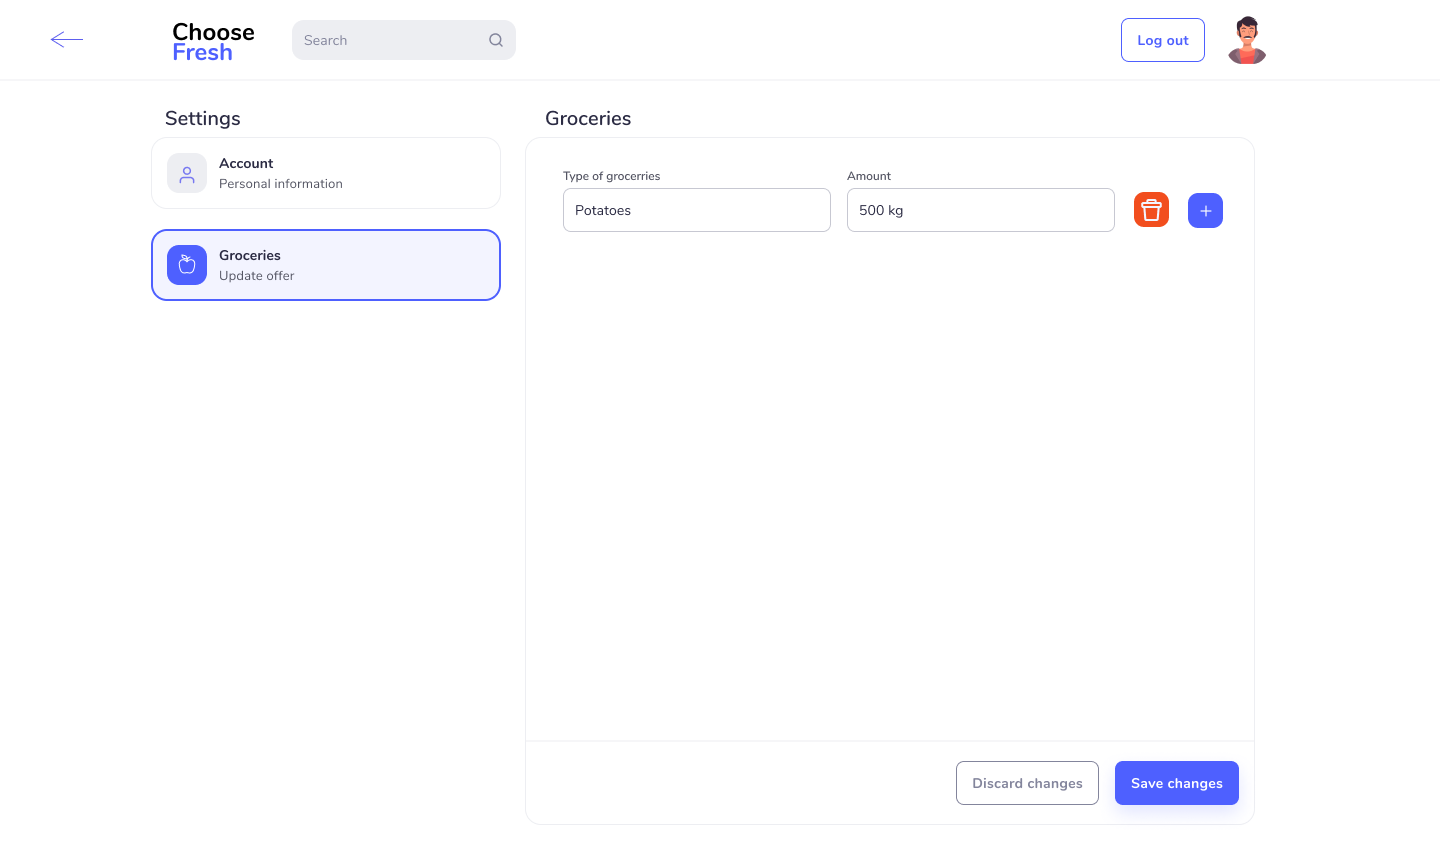
\includegraphics[width=\textwidth]{UI/Supplier Groceries Update (Screen 1).png}
    		\caption{Odabir opcije da ažurira namirnice}
    \label{fig:SupplierGroceriesUpdateScreen1}
    \end{center}
\end{figure}

\begin{figure}[H]
	\begin{center}
		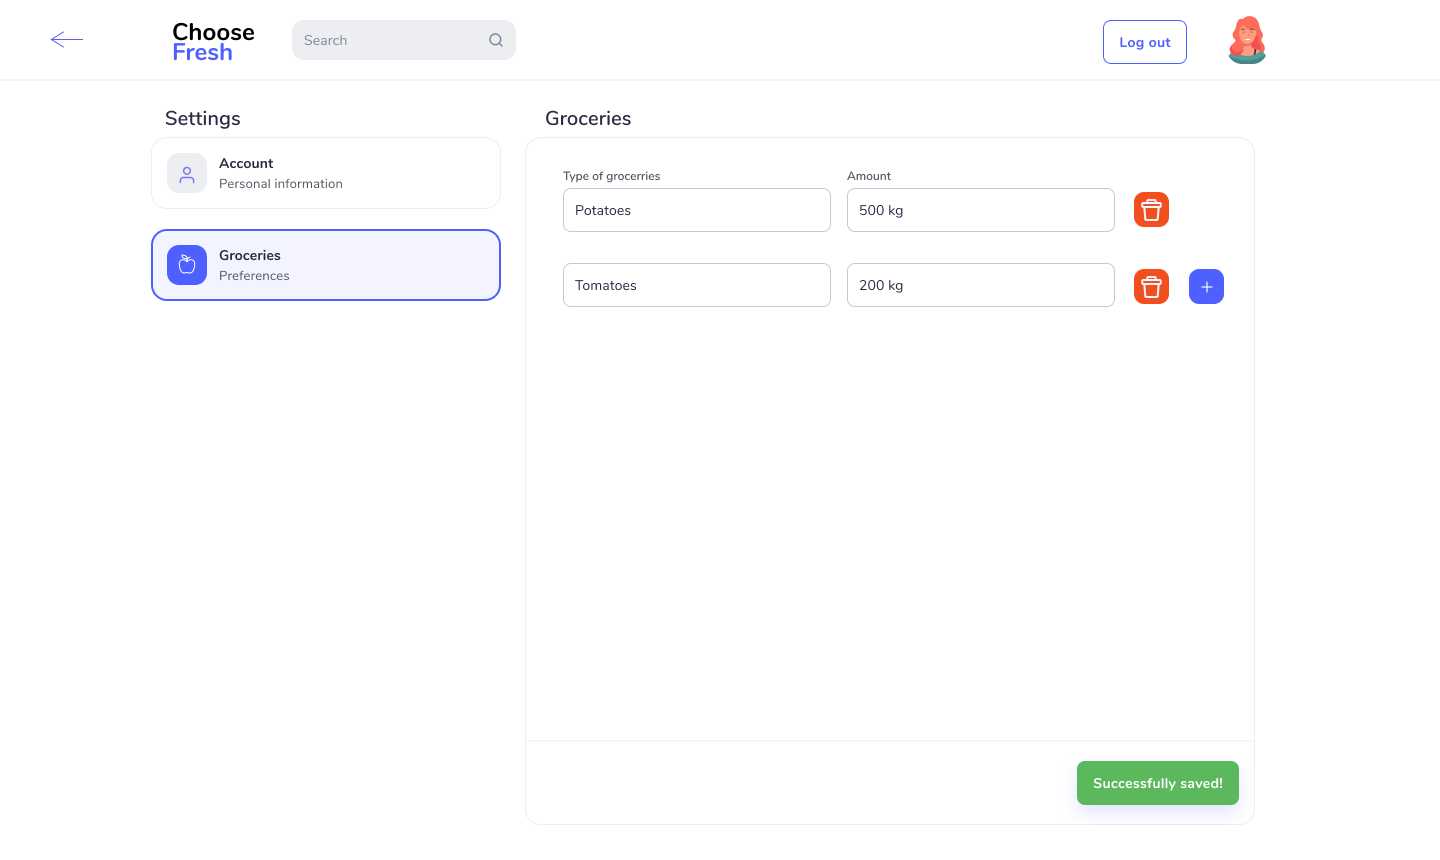
\includegraphics[width=\textwidth]{UI/Supplier Groceries Update (Screen 2).png}
    		\caption{Uspešno ažuriranje namirnica}
    \label{fig:SupplierGroceriesUpdateScreen2}
    \end{center}
\end{figure}
